% Author : Prakash
% Date   : 2022-11-23 16:44
% vim: ai ts=2 sts=2 et sw=2 ft=tex

\documentclass[a4paper,12pt]{article}
\usepackage[margin=30mm]{geometry}

\usepackage{amsmath}
\usepackage{amssymb}
\usepackage{graphicx}
\usepackage{parskip}
\usepackage{tikz}
\usepackage{minted}
\usepackage{hyperref}
\usepackage{pgfplots}
\usepackage{tikz}
\usepackage{multicol}
\usepackage{multirow}

\usetikzlibrary{patterns,plotmarks}


\title{Simulation of helicoil material.}
\author{Prakash Gautam}

\graphicspath{{../../asset}}

%\input{pgf-preamble.tex}

\begin{document}
\maketitle
%The macro used in the primary simulation.
%\inputminted{ini}{../../asset/files/primary-sim-macro.mac}
\section{Primary simulation}
A total of 1000 jobs were submitted of which 988 were completed. This make as a total of 98,800,000 primary events simulated.  The distribution of events that hit the new geometry is shown in Figure \ref{fig:primary-hit-det}. The total events that hit helicoil material (across all simulated files) is: 2091094 (area under the curve in \ref{fig:primary-hit-det}).


\begin{figure}[h!]
    \centering
    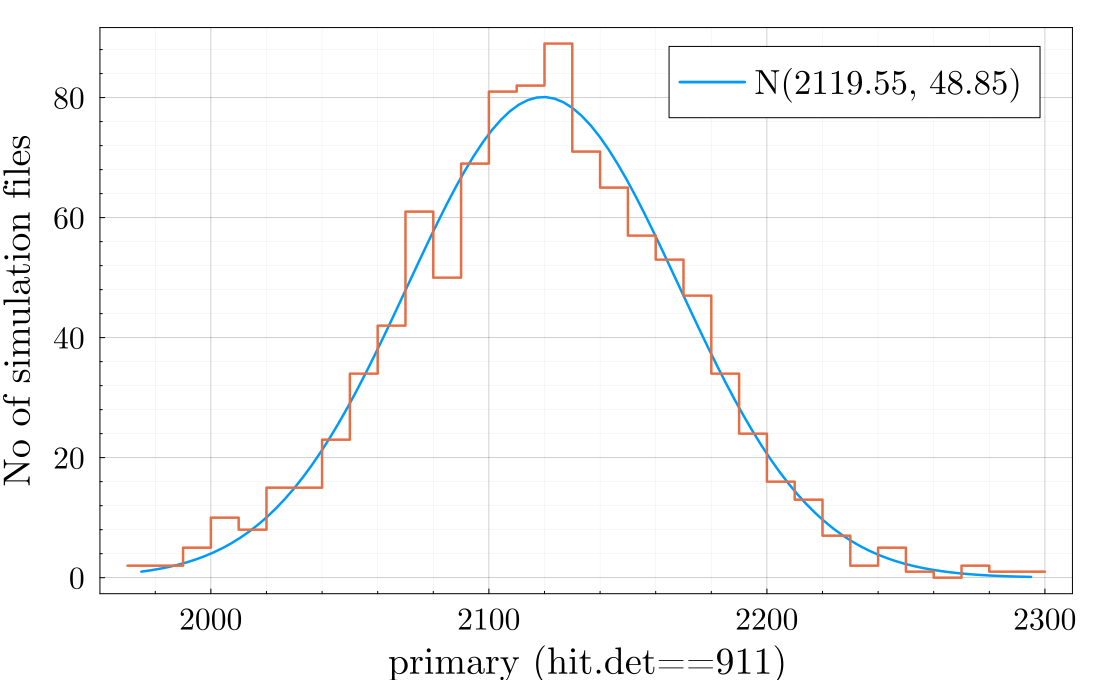
\includegraphics[width=1\linewidth]{image/helicoil-20221121-113016-img-primary-det-hit-count-hist-not-normalized.png}
    \caption{The distribution number of hits helicoil material (hit.det==911). The total primary simulated in each files is 100,000. So only about $0.2$\% make it to the helicoil material. The continuous curve is a gaussian fitted oveer histogram.}
    \label{fig:primary-hit-det}
\end{figure}


These hits can be various different particles. The particle of interest for the secondary is the primary electrons (hit.trid==1).  The distribution of number of hit of these electrons per fileis showin in \ref{fig:primary-dist}. The total electron events hitting the helicoil materials is 10395. This ratio is
\begin{align*}
    \frac{10395}{98800000} = 1.05 \times 10^{-4}
\end{align*}



\begin{figure}[h!]
    \centering
    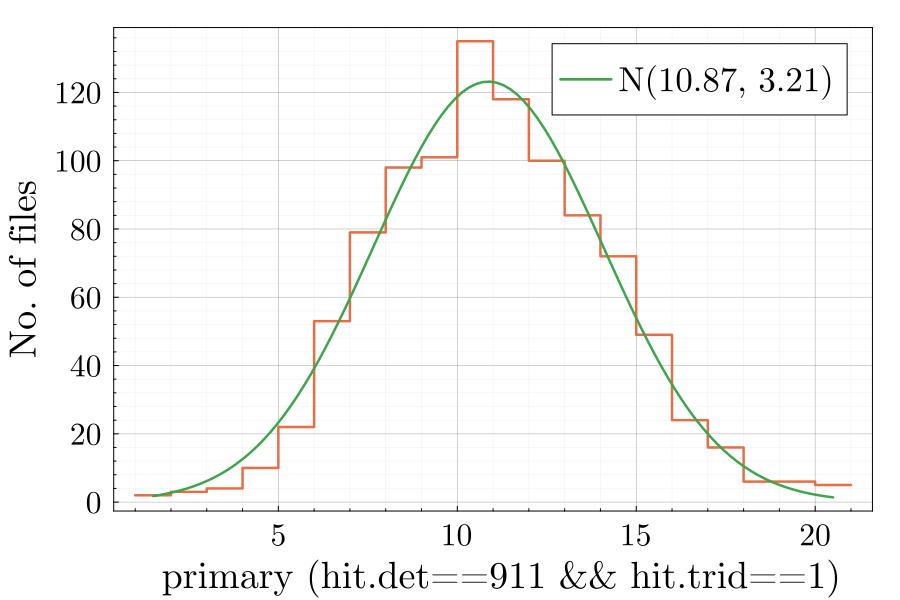
\includegraphics[width=1\linewidth]{image/helicoil-20221121-113016-img-primary-trid-hit-count-hist.png} \caption{The distribution of No. of primary electrons (hit.trid==1) that hit the new geometry (hit.det ==911).}
    \label{fig:primary-dist}
\end{figure}

All of these simulated files is combined into a single primary ``Skimmed" root tree containing only the hit branch with "hit.trid==1 \&\& hit.det==911" (here 911 corresponds to the detector id for the helicoil geometry).

\section{Secondary simulation} \label{sec:secondary-simulation}
With this skimmed file as an input generator to the simulation, a total 100 secondary simulation is run with 100,000 events each. One of the jobs failed with 99 complete jobs. It amounts the simulation of 9,900,000 secondary events.
\begin{figure}[h!]
    \centering
    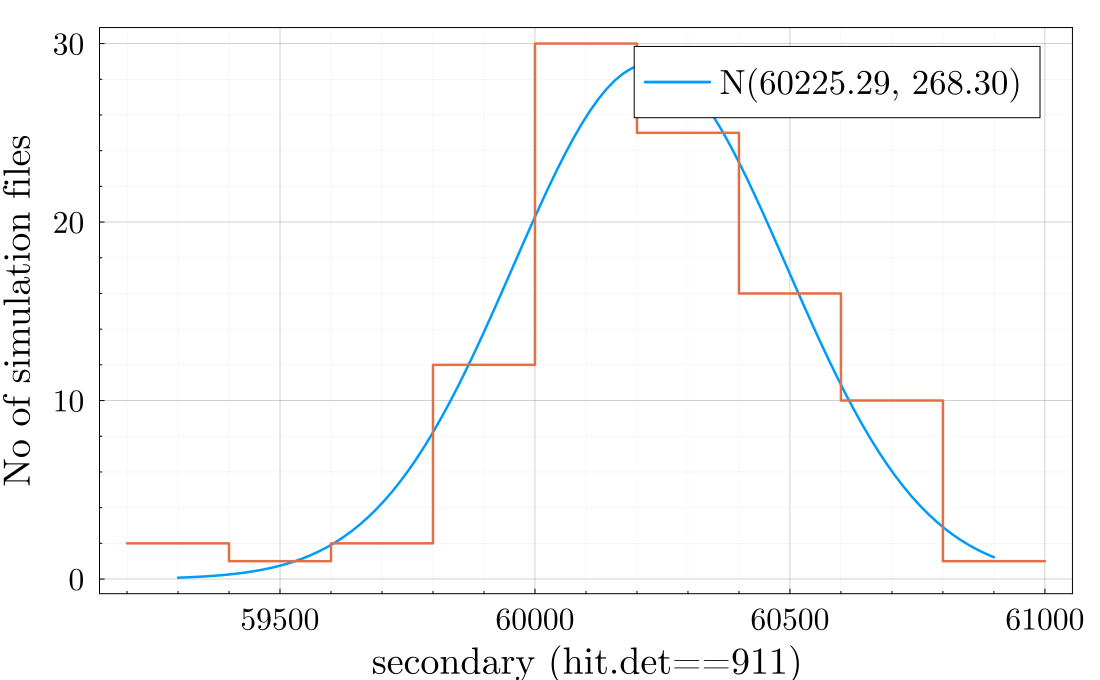
\includegraphics[width=1\linewidth]{image/helicoil-20221121-113016-img-secondary-det-hit-count-hist-not-normalized.png}
    %\input{../../asset/image/helicoil-20221121-113016-img-113016-secondary-det-hit-count-hist-not-normalized.tex}
    \caption{The distribution of hit in the helicoil geometry for secondary simulation. Only $\sim 60$\% of the events hit the new geometry.}
    \label{fig:sec-hit-det-distrib}
\end{figure}

The distribution of hits in the secondary simulation files is shown in Figure \ref{fig:sec-hit-det-distrib}.

\begin{figure}[h!]
    \centering
    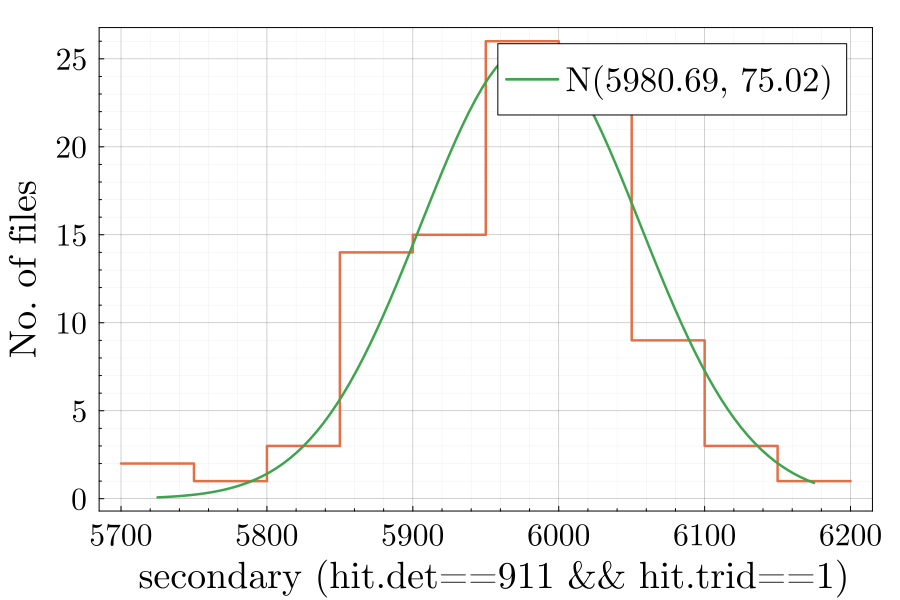
\includegraphics[width=1\linewidth]{image/helicoil-20221121-113016-img-secondary-trid-hit-count-hist.png}
    \caption{The distribution of No. of electrons (hit.trid==1) that hit the new geometry (hit.det ==911)}
    \label{fig:sec-hit-911-trid-1}
\end{figure}

For the final detector the event distribution is shown in Figure \ref{fig:sec-hit-28-no-trid}.
\begin{figure}[h!]
    \centering
    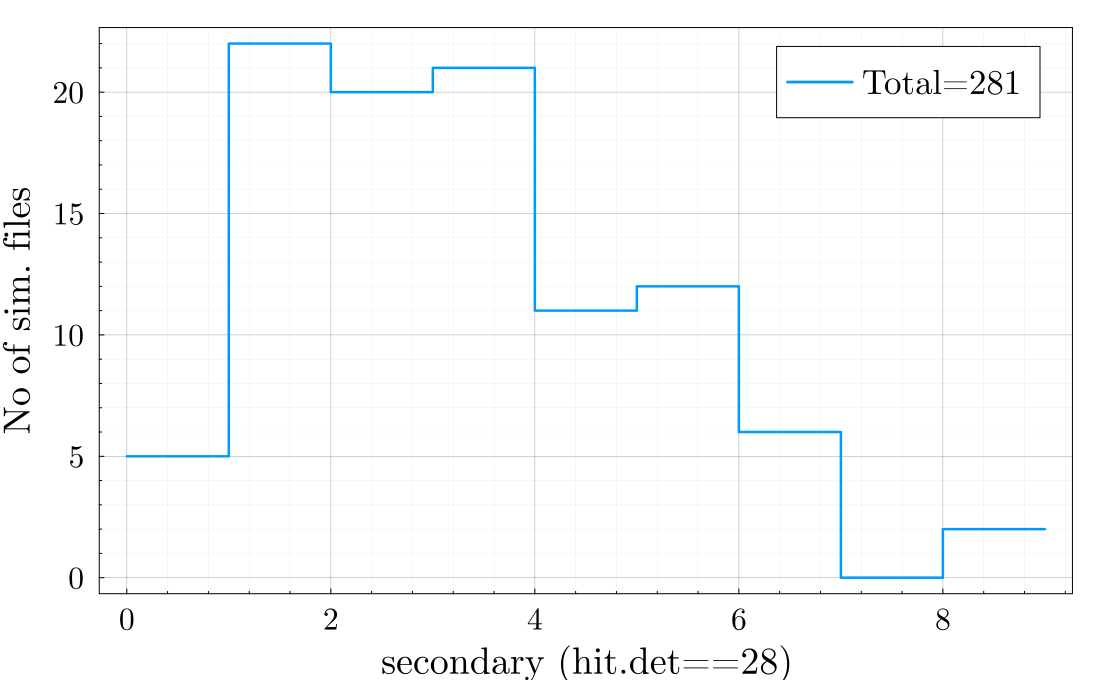
\includegraphics[width=0.9\linewidth]{image/helicoil-20221121-113016-secondary-fin-det-hit.png}
    \caption{The distribution of number of events per 100,000 secondary simulation in the final detetector (hit.det==28). A total of 281 events make it to the detector, of the total simulated 9,900,000 secondary events.}
    \label{fig:sec-hit-28-no-trid}
\end{figure}
\begin{align*}
    \frac{281}{9900000} = 2.83 \times 10^{-5}
\end{align*}
\subsection{Energy distribution}
All of the secondary simulation files are combined into a single root file.
\begin{table}[h!] \label{tab:energy-distrib}
    \centering
    \caption{Energy distribution of events hit in the primary simulation and secondary simulation. The secondary simulation uses the events selected from primary with cut (hit.det==911 \&\& hit.trid==1)}
    \begin{tabular}{r|r|rr}
            &  Primary($9.88 \times 10^{7}$)  &  \multicolumn{2}{c}{Secondary($9.9 \times 10^{6}$)} \\
            \hline
        Energy[hit.e] (MeV) & det==911\&\& trid==1  &  det==911 &  det == 28 \\
        \hline \hline
        0.00 - 0.01         &    0 &   931465&     0 \\ % previous version had 36 energy interval changed () --> [)
        0.01 - 0.10         &    0 &  191606 &   182 \\
        0.10 - 1.00         &   11 & 3876080 &    85 \\
        1.00 - 10.00        &  829 &  889937 &    10 \\
        10.00 - 100.00      & 9018 &   66011 &     2 \\
        100.00 - 1000.00    &  432 &    6026 &     2 \\
        1000.00 - 100000.00 &  104 &      61 &     0 \\
        \hline
        Total               & 10394 &5961186 &   281\\
        \hline \hline
    \end{tabular}
\end{table}

\section{Problem}
    As described in  Section \ref{sec:secondary-simulation} the generator used for the secondary simulation is the ``skimmed" primary which only has those primary electron events (trid==1) which hit the added geometry (hit.det==911). It is expected that each registered event in the secondary hit the added geometry (911). But apparantly the Figure \ref{fig:sec-hit-det-distrib} seems to suggest that it is not the case. We would expect that 100\% of the simulated events hit the new detector by definition.

    This confusion is because of the way we are counting events. A remoll simulation file has a data structure like this

\begin{minted}[autogobble]{markdown}
                     FILE1.root                               FILE2.root
             SN.   rate          hit                  SN.   rate          hit
            +-----+-------------+---------           +-----+-------------+---------
            1.    41.00         [911]                1.    41.00         [911,28]
            2.    41.00         [911,28]             2.    41.00         [911,911]
            3.    41.00         []                   3.    41.00         []
            4.    41.00         []                   4.    41.00         []
            5.    41.00         [911,911]            5.    41.00         []    
        \end{minted}

    Say we have two simulation files ``FILE1.root" and ``FILE2.root". We can see that for some simulated events there are no hits registered. So to see all the events on each file, I wrote a script that reads each events and inspects each hit vector for each secondary simulation data. For the 99 files that were simulated in the secondary on an average $\sim 63$\% of the simulated events did not register any hit on either the new geometry added (hit.det==911) or the detector (hit.det==28). 
    \begin{figure}[h!]
        \centering
        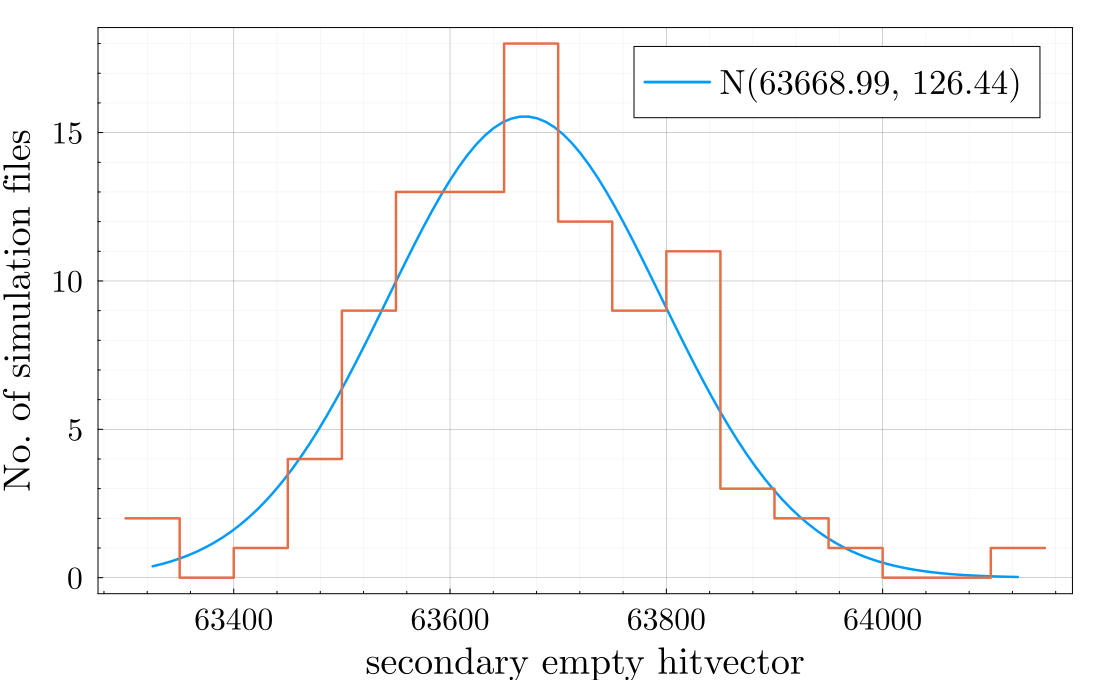
\includegraphics[width=1\linewidth]{image/helicoil-20221121-113016-inspect-secondary-empty-hitvec-distrib.png}
        \caption{The number of simulated events out of $1 \times 10^{5}$ that did not register hit in either the new geometry or the MOLLER detector.}
        \label{fig:inspect-empty-hitvec-distrib}
    \end{figure}


    When these two files are merged into a single secondary file, I take the average of rate and merge the hit one by one like:
        \begin{minted}[autogobble]{markdown}
                     Merged file
             SN.   rate          hit
            +-----+-------------+-----
            1.    41.00         911   --+---> FILE1.root SN. 1
            2.    41.00         911   --+---> FILE1.root SN. 2
            3.    41.00         28    __|
            4.    41.00         911   --+---> FILE1.root SN. 5
            5.    41.00         911   __|
            6.    41.00         911
            7.    41.00         28
            8.    41.00         911   --+---> FILE2.root SN. 2
            9.    41.00         911   __|
        \end{minted}

    The number I reported in Section \ref{sec:secondary-simulation} uses a merged file like the one above. With this file it seems that the rate of new geometry hit in the secondary simulation is 7 out of the total 10 (5+5) that we simulated. However the correct way to merge these files should have been. 

        \begin{minted}[autogobble]{markdown}
                     Merged.root           
             SN.   rate          hit       
            +-----+-------------+--------- 
            1.    41.00         [911]      
            2.    41.00         [911,28]   
            3.    41.00         [911,911]  
            4.    41.00         [911,28]
            5.    41.00         [911,911]
        \end{minted}

   And this shows that there is at least a hit to the new geometry added for each event that registered at least one hit. 

   If we go by this way then the ``Hit Summary" of the two files we simulated can be written as:
   \begin{minted}[autogobble]{python}
        Simulated: 10
        Empty    : 5
        Nonempty : 5
        Hit@28   : 1
        Hit@911  : 7
        Miss@911 : 0
   \end{minted}

   For the 99 secondary simulation files this statistics is:

   \begin{minted}[autogobble]{python}
        Simulated: 9,900,000
        Empty    : 6,303,843
        Nonempty : 3,596,157
        Hit@28   : 281
        Hit@911  : 5,961,186
        Miss@911 : 0
   \end{minted}

These numbers match to the one I obtained in the energy distribution table \ref{tab:energy-distrib}.


%test\cite{qianNeutrinoMassHierarchy2015}
%\bibliographystyle{ieeetr85}
%\bibliography{Neutrino.bib}
\end{document}

